\documentclass[11pt,a4paper]{article}
\usepackage[margin=2.2cm]{geometry}
\usepackage{amsmath,amssymb}
\usepackage{siunitx}
\usepackage{booktabs}
\usepackage{xcolor}
\usepackage{microtype}
\usepackage{enumitem}
\usepackage{tcolorbox}
\usepackage{graphicx}
\definecolor{ink}{HTML}{14231B}\definecolor{accent}{HTML}{0F3D2A}
\tcbuselibrary{skins}
\newtcolorbox{key}{colback=accent!6,colframe=accent,boxrule=0.6pt,arc=2pt,left=6pt,right=6pt,top=4pt,bottom=4pt}
\sisetup{per-mode=symbol,group-separator={\,}}
\setlength{\parindent}{0pt}\setlength{\parskip}{6pt}
\renewcommand{\arraystretch}{1.25}

\title{\textbf{Slide 13: verification and next steps}\\\large What the simulation proves and what is still open}
\author{ADS7057 test board v3 \quad ---\quad study notes}\date{}
\begin{document}\maketitle\vspace{-1.2em}
\section{How it is checked}
\begin{center}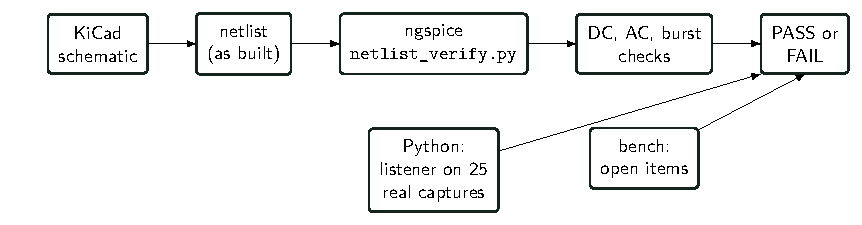
\includegraphics[width=0.98\textwidth]{s13_circuit.pdf}\end{center}
\texttt{sim/netlist\_verify.py} reads the KiCad netlist of the board as built, so a wrong net or value shows up. It builds an ngspice circuit with vendor models and runs a DC operating point, an AC sweep and a burst test. A second script runs the listener thresholds on 25 real captures.

\section{Results}
\begin{center}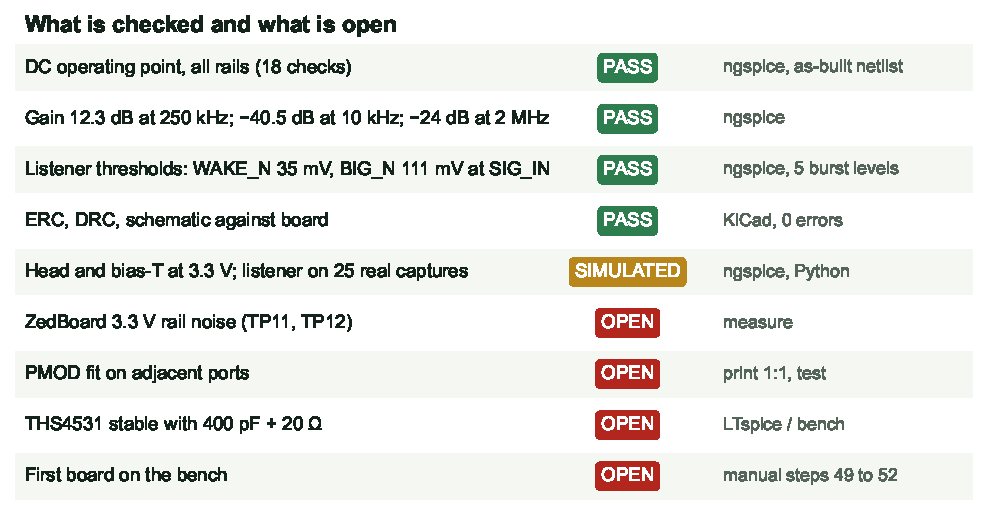
\includegraphics[width=0.95\textwidth]{s13_graph.pdf}\end{center}
\begin{center}\begin{tabular}{lrr}\toprule Check & Result & Limit\\\midrule
All 18 DC nodes (rails, mid-rails, ladder) & within limits & $\pm1$ to 3\,\%\\
Gain SENSOR IN to ADC at \SI{250}{kHz} & \SI{12.28}{dB} & 11.5 to 13\\
Loss at \SI{10}{kHz} and \SI{2}{MHz} & \SI{40.5}{dB}, \SI{24.0}{dB} & 38 to 50, 18 to 40\\
Current from the PMOD & \SI{24.8}{mA} & 15 to 40\\
Burst, \SI{45}{mV} generator & WAKE\_N low, BIG\_N high & as designed\\
Burst, \SI{112}{mV} generator & both low & as designed\\
\bottomrule\end{tabular}\end{center}
\textbf{Result: all pass.} The simulation proves that the netlist does what the design intends. It does not prove the real parts, the layout or the sensor spectrum.

\section{Open items, in order of risk}
\begin{enumerate}[leftmargin=1.4em]
\item \textbf{THS4531 with \SI{400}{pF} and \SI{20}{\ohm}.} The datasheet expects about \SI{2}{pF} between the outputs. Stability with this load is not confirmed yet. Run the LTspice netlist, then look at an output step on the bench.
\item \textbf{Anti-aliasing margin.} Only \SI{8}{dB} at \SI{800}{kHz} (slide 6). Measure the real sensor spectrum with the new head.
\item \textbf{Listener margin.} Noise peak \SI{26}{mV} against \SI{35}{mV}. Set the thresholds from bench data.
\item \textbf{ZedBoard 3.3 V rail noise} (TP11, TP12) and the \textbf{PMOD fit} on adjacent ports (print 1:1).
\item \textbf{ADC decoupling:} the \SI{100}{nF} DVDD capacitor is \SI{4.5}{mm} from the pin.
\item \textbf{Manual fixes:} the head test text says VREF settles in \SI{0.2}{s}; with a $1\,$M$\Omega$ divider it takes about \SI{25}{s}. The driver input corner is \SI{119}{Hz}, not \SI{159}{Hz} (slide 7).
\end{enumerate}

\section{Next steps}
\begin{enumerate}[leftmargin=1.4em]
\item Bring-up in this order: rails (manual step 49), a \SI{250}{kHz} burst at J1 (step 50), the response sweep (51), the listener (52).
\item Scale to 16 channels with the backplane (FMC adapter and two 8-slot modules, in \texttt{hw/backplane/}). Open items there: JLC placement of the FMC plug, card guides, SCLK integrity.
\item FPGA side: a scheduler for the two modes (continuous sampling of a few plants, wake-up of all 16).
\end{enumerate}
\end{document}
